\documentclass[english]{article}
\usepackage{style,macros}
\bibliography{sources}

\numberwithin{equation}{section}

\title{Revisiting the topological Lefschetz fixed point theorem}
\author{Oscar Harr \and Florian Riedel}

\begin{document}

\maketitle

\tableofcontents

\subsection{Bartels--Nikolaus assembly morphisms}
Here we give a brief account of the Bartels--Nikolaus theory of abstract assembly morphisms associated to copairings in a symmetric monoidal category. Throughout this section, fix a symmetric monoidal category $\mathcal C$. We assume that $\mathcal C$ is {\em closed}, meaning that for each $X\in\mathcal C$, the functor
$$
{-}\otimes X\colon\mathcal C\to\mathcal C
$$
has a right adjoint that we denote
$$
\Hom_{\mathcal C}(X,{-})\colon\mathcal C\to\mathcal C.
$$
We refer to the counit of this adjunction as {\em evaluation}, and denote it by
$$
\evalu_X\colon X\otimes\Hom_{\mathcal C}(X,{-})\to\text{id}_{\mathcal C}.
$$
\begin{defn}[Bartels--Nikolaus]
  Let $A$ and $B\in\mathcal C$, and let $\delta\colon\mathbf 1\to A\otimes B$ be some morphism. The {\em $\delta$-assembly}, denoted $a_{\delta}$, is defined by the following string diagram:
  \begin{equation*}
    \label{eq:assembly}
    a_\delta =
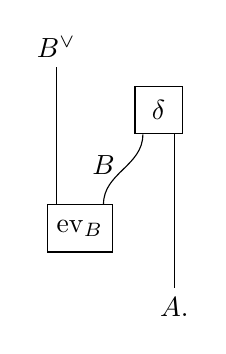
\begin{tikzpicture}[baseline=(current bounding box.center)]
  % Nodes
  \node (Bvee) at (-0.3,3.3) {$B^\vee$};
  \node (deltabox) at (1,2.5) [rectangle, draw, minimum width=0.6cm, minimum height=0.6cm] {$\delta$};
  \node (evbox) at (0,1) [rectangle, draw, minimum width=0.6cm, minimum height=0.6cm] {$\mathrm{ev}_B$};
  \node (A) at (1.2,0) {$A$.};
  \node (B) at (0.3,1.8) {$B$};

  % Edges
  \draw (Bvee) -- (evbox.north -| -0.3,1.3);
  \draw (deltabox.south -| 0.8,2.5) to [out=270,in=90] (evbox.north -| 0.3,1.3);
  \draw (deltabox.south -| 1.2,2.5) -- (A);
  \end{tikzpicture}
\end{equation*}
\end{defn}
Now let $\mathcal D$ be another closed symmetric monoidal category, and let $F\colon\mathcal C\to\mathcal D$ be a symmetric monoidal functor.
\begin{defn}
  For each $X\in\mathcal C$, let $\eta (X)\colon F(X^\vee )\to\Hom_{\mathcal D}(F(X),F(\mathbf 1))$ denote the tensor-Hom adjoint of the composition
  $$
  F(X^\vee)\otimes F(X)\xrightarrow\sim F(X^\vee\otimes X)\to F(\mathbf 1);
  $$
  that is, $\eta (X)$ is defined by the equation
  \begin{equation}
    \label{eq:eta-defn}
    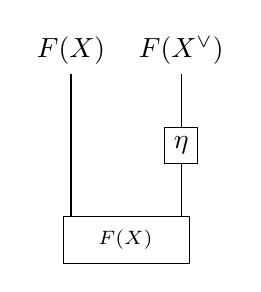
\begin{tikzpicture}[baseline=(current bounding box.center)]
  % Nodes
  \node (X) at (-0.7,3) {$F(X)$};
  \node (Xvee) at (0.7,3) {$F(X^\vee)$};

  \node[rectangle, draw,minimum width=0.4cm, minimum height=0.4cm] (etabox) at (0.7,1.8){$\eta$};

  % Evaluation box
  \node[rectangle, draw, minimum width=1.6cm, minimum height=0.6cm] 
  (evFbox) at (0,0.6) {$\evalu_{F(X)}$};

  % Edges
  \draw (X) to (evFbox.north -| -0.7,2.5);
  \draw (Xvee) to (etabox.north);
  \draw (etabox.south) to (evFbox.north -| 0.7,2.5);
\end{tikzpicture}
=
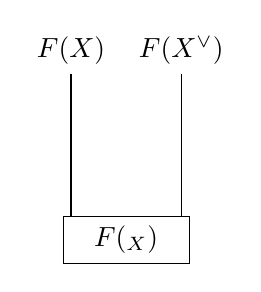
\begin{tikzpicture}[baseline=(current bounding box.center)]
  % Nodes
  \node (X) at (-0.7,3) {$F(X)$};
  \node (Xvee) at (0.7,3) {$F(X^\vee)$};

  % Evaluation box
  \node[rectangle, draw, minimum width=1.6cm, minimum height=0.6cm] 
  (evFbox) at (0,0.6) {$F(\evalu_{X})$};

  % Edges
  \draw (X) to (evFbox.north -| -0.7,0);
  \draw (Xvee) to (evFbox.north -| 0.7,0);
\end{tikzpicture}
\end{equation}
\end{defn}
\begin{prop}[Bartels--Nikolaus]
  Let $F\colon\mathcal C\to D$ be a symmetric monoidal functor between closed symmetric monoidal categories, and let $A$ and $B\in\mathcal C$.  There is a commutative diagram
  $$
  \begin{tikzcd}
    F(B^\vee )\arrow[rr,"F(a_\delta )"] \arrow[rd,"\eta (B)"]&& F(A) \\
    & \operatorname{Hom}_{\mathcal D}(F(B),F(\mathbf 1))\arrow[ru]
  \end{tikzcd}
  $$
\end{prop}
In fact, Bartels and Nikolaus assume only that $F$ is {\em lax} symmetric monoidal. 
\begin{proof}
  We have
    \begin{equation*}
    \label{eq:assembly}
    F(a_\delta) \quad =
    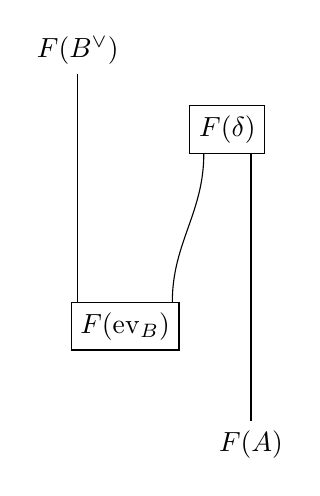
\begin{tikzpicture}[baseline=(current bounding box.center)]
      % Nodes
      \node (Bvee) at (-0.6,4) {$F(B^\vee)$};
      \node (A) at (1.6,-1) {$F(A)$};

      \node (deltabox) at (1.3,3) [rectangle, draw, minimum width=0.6cm, minimum height=0.6cm] {$F(\delta )$};
      \node (evbox) at (0,0.5) [rectangle, draw, minimum width=0.6cm, minimum height=0.6cm] {$F(\mathrm{ev}_B)$};


      % Edges
      \draw (Bvee) -- (evbox.north -| -0.6,1.3);
      \draw (deltabox.south -| 1,2.5) to [out=270,in=90] (evbox.north -| 0.6,1.3);
      \draw (deltabox.south -| 1.6,2.5) -- (A);
    \end{tikzpicture}
    =
        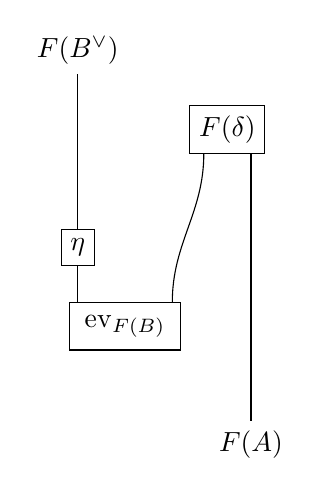
\begin{tikzpicture}[baseline=(current bounding box.center)]
      % Nodes
      \node (Bvee) at (-0.6,4) {$F(B^\vee)$};
      \node (A) at (1.6,-1) {$F(A)$};

      \node (etabox) at (-0.6,1.5) [rectangle, draw, minimum width=0.4cm, minimum height=0.4cm]{$\eta$};
      \node (deltabox) at (1.3,3) [rectangle, draw, minimum width=0.6cm, minimum height=0.6cm] {$F(\delta )$};
      \node (evbox) at (0,0.5) [rectangle, draw, minimum width=1.4cm, minimum height=0.6cm] {$\mathrm{ev}_{F(B)}$};


      % Edges
      \draw (Bvee) -- (etabox.north);
      \draw (etabox.south) -- (evbox.north -| -0.6,1.3);
      \draw (deltabox.south -| 1,2.5) to [out=270,in=90] (evbox.north -| 0.6,1.3);
      \draw (deltabox.south -| 1.6,2.5) -- (A);
    \end{tikzpicture}
        =
        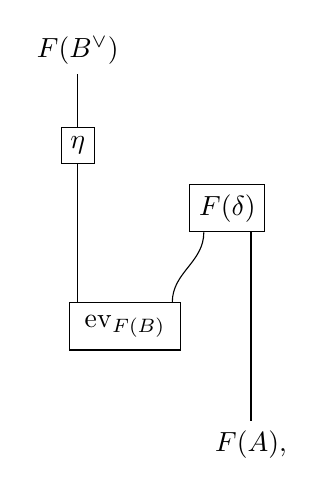
\begin{tikzpicture}[baseline=(current bounding box.center)]
      % Nodes
      \node (Bvee) at (-0.6,4) {$F(B^\vee)$};
      \node (A) at (1.6,-1) {$F(A)$,};

      \node (etabox) at (-0.6,2.8) [rectangle, draw, minimum width=0.4cm, minimum height=0.4cm]{$\eta$};
      \node (deltabox) at (1.3,2) [rectangle, draw, minimum width=0.6cm, minimum height=0.6cm] {$F(\delta )$};
      \node (evbox) at (0,0.5) [rectangle, draw, minimum width=1.4cm, minimum height=0.6cm] {$\mathrm{ev}_{F(B)}$};


      % Edges
      \draw (Bvee) -- (etabox.north);
      \draw (etabox.south) -- (evbox.north -| -0.6,1.3);
      \draw (deltabox.south -| 1,2.5) to [out=270,in=90] (evbox.north -| 0.6,1.3);
      \draw (deltabox.south -| 1.6,2.5) -- (A);
  \end{tikzpicture}
\end{equation*}
as desired.
\end{proof}
\end{document}
